\section{Gyroscope}\label{section:gyroscope}
%hvad er det?
%hvordan virker det. vis tegning.
%hvad kan det bruges til?
%hvad er drifting. hvorfor drifter den? hvordan fixer man det? PIETER JAN!

The gyroscope measures the rotational velocity ($rad/s$), meaning how much the orientation of the phone has changed since last reading.
The orientations of the phone is referred to as \textit{Pitch}, \textit{Roll}, and \textit{Yaw} and is measured around the axes x, y, and z, respectively as illustrated in \figref{figure:phone-gyroscope}. 
As an example, if the user rotates the device $20^\circ$ around its x-axis, Pitch will, over the course of the action, accumulate to $0.35$ radians, whereas Roll and Yaw remain unaffected.

\begin{figure}[h]
	\centering
	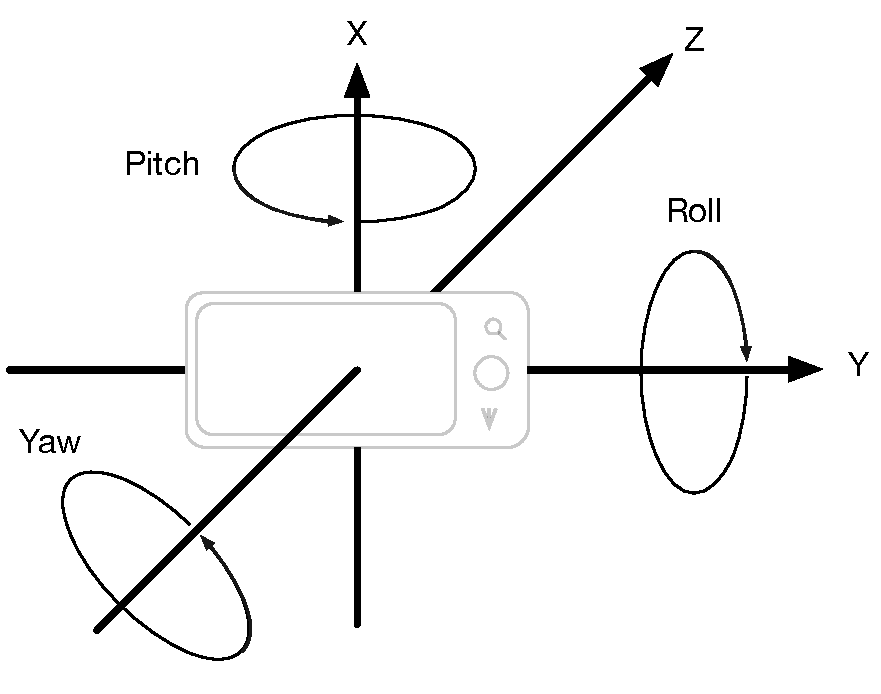
\includegraphics[scale=0.5]{media/phone-rotation/phone-gyroscope}
	\caption{Pitch, Roll and Yaw illustrated.}
	\label{figure:phone-gyroscope}
\end{figure}

The gyroscope can be used in the application to accommodate for tilting the phone while playing.
Without this accommodation the gravitational pull would affect the acceleration-reading of the y-axis, when the phone has a yaw-rotation.
Furthermore, if the phone has a pitch-rotation, the acceleration in the y-axis is smaller than intended, which can be corrected using the gyroscope and is further explained in \secref{section:SensorFusion}.

When using the gyroscope, the accumulation of each gyroscope reading is needed to determine the correct angle that the phone is tilted. 
Due to noise in the gyroscope readings, the accumulated value will be inaccurate.
The inaccuracy can cause drifting, which means the gyroscope cannot track when the system is back to its original position.
To avoid drifting, the gyroscope can be utilised together with the accelerometer to correct the uncertainties of the gyroscope \citep{misc:pieter-jan, misc:balance-filter}.

To test how much the angle drifts, the device was positioned on a flat, undisturbed surface for 3 minutes.
The recording can be seen in \figref{figure:phone-complementary-filter} where one graph illustrates raw data received from the gyroscope, and another graph illustrates the same dataset run through a complementary filter.

\begin{figure}[h]
	\centering
	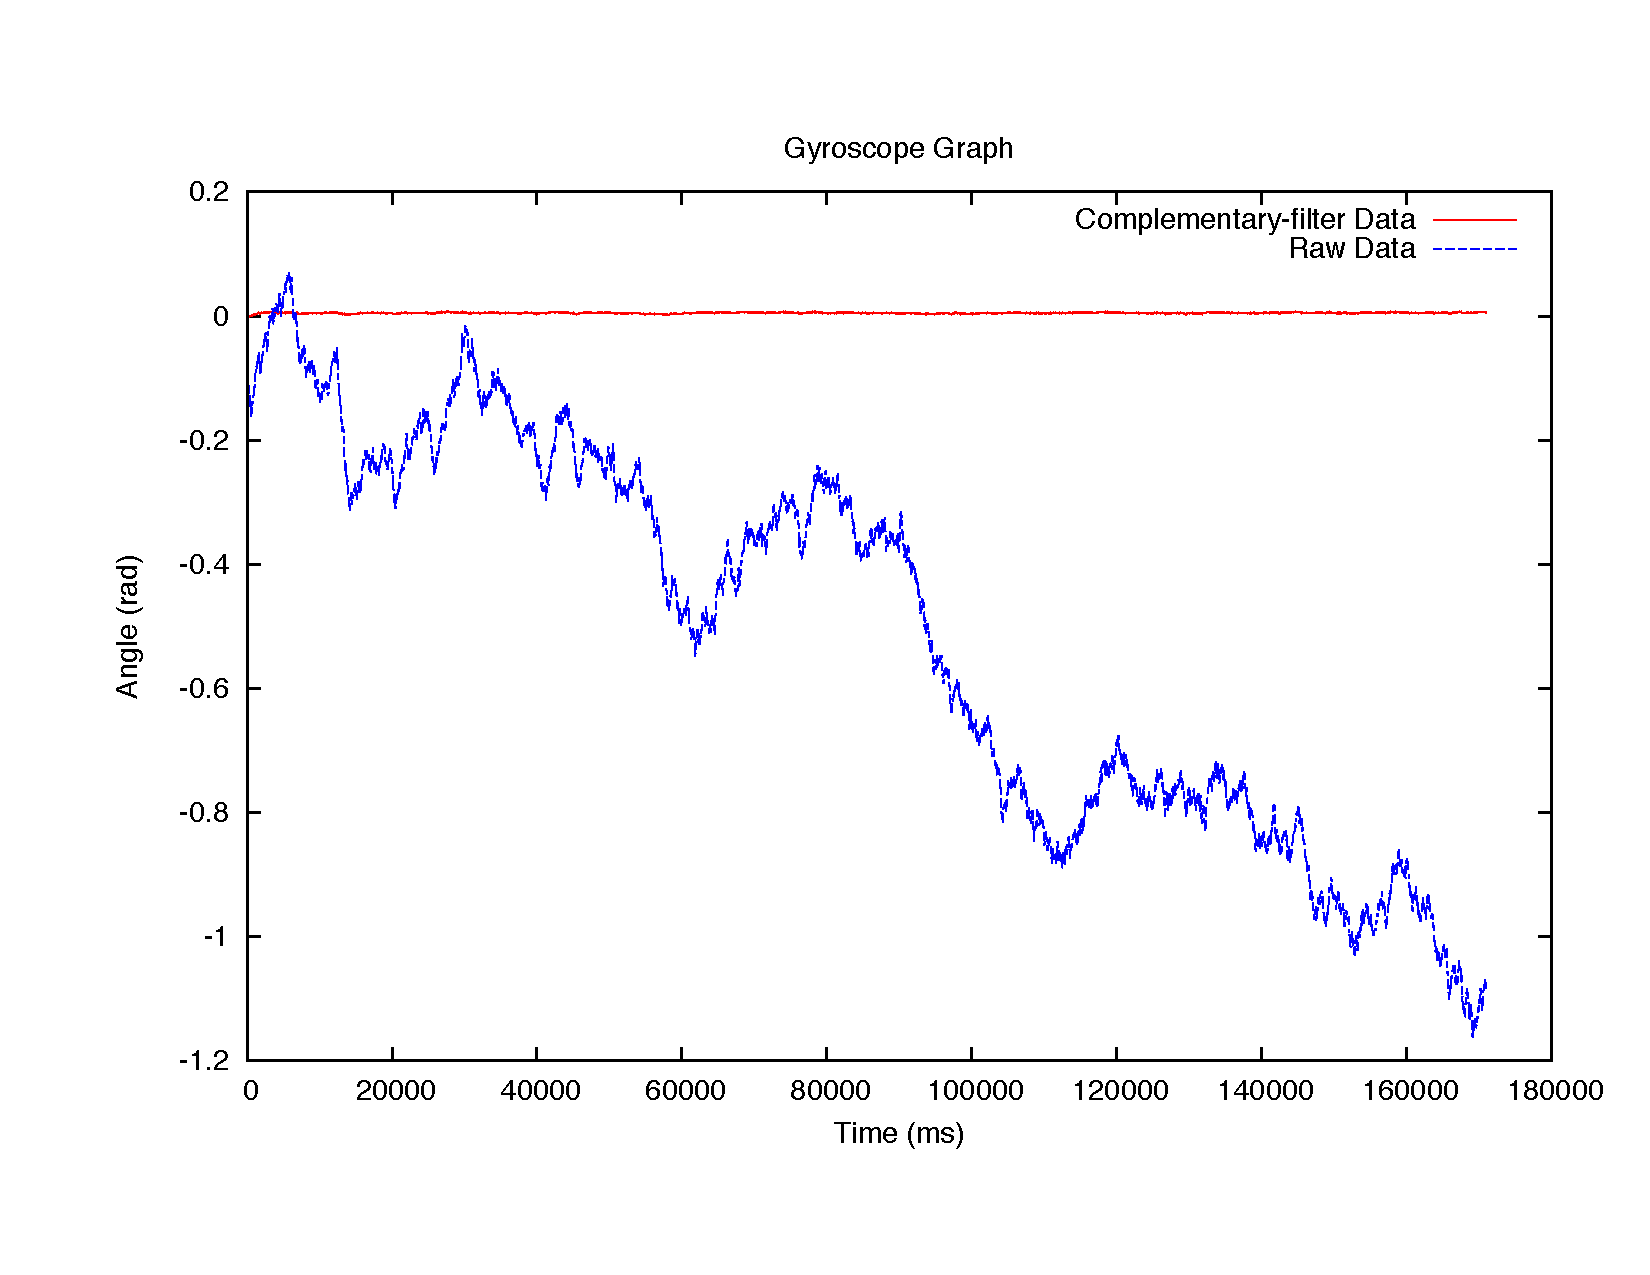
\includegraphics[scale=0.45, trim = 0cm 2cm 0cm 2cm]{media/gnuplot/compfilter.pdf}
	\caption{The complementary-filter over a 3 minute period.}
	\label{figure:phone-complementary-filter}
\end{figure}

As is clearly evident by the graphs, implementing a complementary filter would greatly increase the accuracy of the application.
The sensor fusion is implemented using a complementary filter to have the acceleration reading adjust the accumulated angle of the gyroscope.
The formula is as follows:

\begin{equation*}
	angle = \alpha*(angle + gyro * \Delta t) + (1 - \alpha)(angle_{acc})
\end{equation*}
where,
\begin{enumerate}
	\item[]
\begin{enumerate}
	\item[$angle$] is the accumulated angle.
	\item[$\alpha$] is the coefficient which determine how much each sensor affects the result.
	\item[$gyro$] is the gyroscope reading measured in $rad/s$.
	\item[$angle_{acc}$] is the angle, determined by the acceleration, measured in $rad$ and found using atan2 function.
\end{enumerate}
\end{enumerate}
